\documentclass[11pt,a4paper]{article}
\usepackage{graphicx}
\usepackage{amsmath,amssymb,amsthm,amsfonts}
\usepackage{geometry}\geometry{left=2.3cm,right=2.3cm,top=2.5cm,bottom=2.5cm}
\usepackage{setspace}\setstretch{1.20}
\usepackage{hyperref}\hypersetup{colorlinks=true,linkcolor=black,citecolor=black}
\usepackage{parskip,booktabs,array,xcolor,titlesec,enumitem}
\titleformat{\section}{\large\bfseries}{}{0em}{}[\titlerule]
\titlespacing{\section}{0pt}{14pt}{6pt}
\titleformat{\subsection}{\normalsize\bfseries}{\thesubsection\;}{0em}{}
\newtheorem{remark}{Remark}
\begin{document}
\begin{center}
{\LARGE\bfseries Numerical Protocol}\\[0.3cm]
{\large Leverage Effect Evaluation\\
under a Heston Model with Strong Leverage}\\[0.2cm]
{\normalsize Othmane Zarhali}
\end{center}
\vspace{0.15cm}\noindent\rule{\textwidth}{0.8pt}

\begin{abstract}

The leverage-effect experiment is conducted according to the following
steps:

\begin{enumerate}
    \item \textbf{Reference property.} Consider the leverage effect,
    defined as the negative correlation between current returns and
    future variance,
    \[
    \mathrm{Corr}(r_t,V_{t+L})<0,
    \]
    whereby a negative return today is associated with an increase in
    future volatility.

    \item \textbf{Data generation.} Simulate a Heston
    stochastic-volatility data-generating process (DGP) under two
    strong-leverage scenarios:
    \[
    \rho=-1.00
    \qquad\text{and}\qquad
    \rho=-0.80,
    \]
    corresponding respectively to perfect negative correlation and a
    strong leverage level representative of the upper end of typical
    equity-index calibrations.

    \item \textbf{Model calibration.} Calibrate three stochastic
    volatility models to the stylised-fact profile of the Heston DGP:
    \begin{itemize}
        \item ESN A2-981003, using its current optimal architecture
        \[
        (N_r,N_z)=(96,12),
        \]
        \item Quadratic Rough Heston (QRH);
        \item Path-Dependent Volatility Guyon--Lekeufack (PDV--GL).
    \end{itemize}

    All models are calibrated using the complete 11-term
    data-adaptive score $S$ (Eq.~\eqref{eq:score}), together with the
    smooth Gaussian-kernel proximity function. The leverage component
    of the score is emphasised through an increased weight
    ($L:1.1\rightarrow3.5$), making it the largest contribution to
    $S$, while simultaneously tightening the leverage-matching
    tolerance.

    \item \textbf{ESN parameterisation.} The ESN read-out consists of
    \begin{itemize}
        \item a linear roughness factor;
        \item a per-mode $z$-bank profile;
        \item a symmetric quadratic interaction term in the reservoir
        state.
    \end{itemize}
    These components are jointly calibrated with the Hurst exponent,
    the reservoir rate bounds, and the output scaling parameter
    (Section~\ref{sec:calib}). No leverage-specific manual tuning is
    introduced during calibration.

    \item \textbf{Model evaluation.} Assess the calibrated models by
    comparing their ability to reproduce the leverage effect across
    both strong-correlation scenarios. The objective is to determine
    whether the ESN's previously observed agreement at
    $\rho=-0.90$ extends throughout the strong-leverage regime.

    Section~\ref{sec:leverage-results} reports three main findings:
    \begin{itemize}
        \item the ESN consistently reproduces approximately
        $70$--$75\%$ of the DGP leverage magnitude for
        $\rho\in\{-1.00,-0.90,-0.80\}$;
        \item the calibrated isotropic quadratic coefficient $m_1$
        remains close to zero in all strong-leverage scenarios,
        indicating that the ESN's intrinsic sign-fixed leverage channel
        already captures most of the effect without requiring the
        quadratic-dilution mechanism previously identified for
        weak-leverage regimes;
        \item QRH predicts the wrong leverage sign at both correlation
        levels, whereas PDV--GL reproduces the correct sign but
        substantially underestimates its magnitude.
    \end{itemize}
\end{enumerate}
\end{abstract}

\tableofcontents\vspace{0.4cm}

\section{DGP: Heston Model at Two Strong-Leverage Levels}
\label{sec:dgp}

The DGP is the classical Heston stochastic-volatility model, simulated
in annualised variance units with a daily time step $dt=1/252$:
\begin{equation}
  dX_t = -\frac{1}{2}V_t\,dt + \sqrt{V_t}\,dt^{1/2}\,dW_t^S,
  \qquad
  dV_t = \kappa(\theta-V_t)\,dt + \xi\sqrt{V_t}\,dt^{1/2}\,dW_t^V,
  \qquad
  \mathrm{Corr}(dW_t^S,dW_t^V)=\rho,
  \label{eq:heston}
\end{equation}
with $\kappa=3.0$ (annualised mean-reversion speed), $\theta=0.04$
(annualised long-run variance, i.e.\ $20\%$ vol), and $\xi=0.35$
(annualised vol-of-vol) held fixed, while $\rho\in\{-1.00,-0.80\}$ is
swept: $\rho=-1.00$ (\textbf{perfect} negative correlation, the
theoretical maximum) and $\rho=-0.80$ (\textbf{strong}, close to the
upper end of a typical equity-index calibration's $\rho\approx-0.6$ to
$-0.7$). The Feller condition $2\kappa\theta\geq\xi^2$ is satisfied
($0.24\geq0.1225$) at both, though simulation still uses a
full-truncation Euler scheme ($V^+=\max(V,0)$ inside both the drift
and diffusion coefficients) for robustness. A large negative return
shock ($dW^S<0$) coincides with a positive variance shock ($dW^V>0$)
whenever $\rho<0$; the size of that co-movement, and hence the
short-lag leverage effect $\mathrm{Corr}(r_t,V_{t+L})$, scales with
$|\rho|$.

\paragraph{Why annualised units.} A naive daily-unit parametrisation
of $(\kappa,\theta,\xi)$ without the $dt=1/252$ conversion understates
$\theta$ relative to $\xi$ by a factor of $\sim252$, badly violating
the Feller condition and collapsing the variance process to zero under
the full-truncation scheme -- this is checked explicitly at
implementation time (\S\ref{sec:mc}).

\section{Models}

All models use Gaussian Brownian innovations. The leverage effect must
\emph{emerge} from each model's own path-dependent or correlated-noise
mechanism, not from asymmetric innovations.

\subsection{ESN A2-981003 (current optimal architecture)}
The ESN's optimal architecture: 7 shared hyperparameters, with
$N_r=96,N_z=12$. \texttt{rough\_scale}, the $z$-readout profile
$(\texttt{zr\_lo},\texttt{zr\_hi})$, and the symmetric quadratic-term
matrix coefficients $(m_1,m_2)$ are calibrated per DGP cell
(\S\ref{sec:calib}), not part of this fixed table.
\begin{table}[h]
\centering
\caption{The 7 shared hyperparameters of the optimal architecture.}
\label{tab:optarch}
\begin{tabular}{@{}lr@{}}
\toprule
Hyperparameter & Value \\
\midrule
$N_r$ & 96 \\
$N_z$ & 12 \\
\texttt{z\_strength} & 0.1929 \\
\texttt{even\_strength} & 2.2291 \\
\texttt{linear\_strength} & 0.1930 \\
\texttt{gamma\_norm} & 0.9651 \\
\texttt{local\_z\_strength} & 0.0476 \\
\texttt{zz\_scale} & 0.0397 \\
\texttt{sign\_prob\_neg} & 0.2219 \\
\texttt{rough\_orientation} & $-1.0$ (fixed) \\
\bottomrule
\end{tabular}
\end{table}
Single $\varepsilon_t\sim\mathcal{N}(0,1)$ drives both return and
reservoir, $\kappa_0<0$ (admissibility, guaranteed by construction
whenever \texttt{rough\_scale}$>0$) -- this fixed negative $\kappa_0$
is the ESN's own \emph{structural} source of a leverage-like effect,
distinct from but exercised by this protocol's calibration to match
the DGP's stronger, correlated-noise leverage mechanism. The volatility
read-out combines three calibrated channels: a linear rough factor
$\texttt{rough\_scale}\cdot q^\top r_t$; a per-mode $z$-bank sum with
weights following a geometric profile
$(\texttt{zr\_lo},\texttt{zr\_hi})$ across the $N_z$ modes; and a
quadratic-in-$r$ term $r_t^\top Qr_t$, $Q=(1/N_r)(m_1I+m_2qq^\top)$ --
a genuine, symmetric $2$-coefficient matrix. All of
\texttt{rough\_scale}, $(\texttt{zr\_lo},\texttt{zr\_hi})$, and
$(m_1,m_2)$ are calibrated per DGP cell, alongside $H$ and the
reservoir rate windows $[\lambda_{\rm lo},\lambda_{\rm hi}]$,
$[a_{\rm lo},a_{\rm hi}]$ (\S\ref{sec:calib}) -- none of these are part
of the shared architecture above.

\subsection{Quadratic Rough Heston (QRH)}
Bourgey \& Gatheral \cite{bourgey2026}: $V_t=Y_t^2+c$, gamma kernel,
Euler-Volterra with 252-step ring buffer. QRH's own leverage mechanism
comes entirely from a single calibrated correlation-like parameter
between its driving noise and the return process; it is calibrated
here exactly as in every other protocol in this line, with no
Heston-specific adjustment.

\subsection{PDV Guyon-Lekeufack (GL)}
Guyon \& Lekeufack \cite{guyon2023}: two-factor power-law kernel,
online from full return history. Leverage in PDV-GL arises from the
model's direct dependence of variance on \emph{signed} past returns
(not just their magnitude), a structurally different mechanism from
both the ESN's fixed-sign reservoir coupling and QRH's single
correlation parameter.

\section{Calibration: Full 11-Term Score, Smooth Kernel}
\label{sec:calib}

\begin{equation}
\begin{aligned}
S &= 2.2\,\bigl(1-f(\hat H)\bigr)+1.4\,\bigl(1-f(\bar\sigma)\bigr)+0.6\,\bigl(1-g(q_{995})\bigr)+0.2\,\bigl(1-g(\sigma_{\max})\bigr)
   +0.8\,\bigl(1-f(\bar V_{\rm ACF})\bigr)\\
  &+1.0\,\bigl(1-f(G_T)\bigr)+0.8\,\bigl(1-f(F_T)\bigr)+1.0\,\bigl(1-f(Z)\bigr)
   +\underbrace{\mathbf{3.5}\,\bigl(1-f(L)\bigr)}_{\text{leverage}}\\
  &+0.7\,\bigl(1-f(K)\bigr)+0.5\,\bigl(1-f(A)\bigr)+5\cdot\mathrm{Stress}.
\end{aligned}
\label{eq:score}
\end{equation}
where $f(x,c,s)=\exp(-\tfrac12((x-c)/s)^2)$,
$g(x,c,s)=\exp(-\tfrac12((x-c)_+/s)^2)$, both in $(0,1]$ (the smooth
Gaussian kernel, replacing a piecewise-linear
tent $\max(0,1-|x-c|/s)$, which has an exactly-zero gradient beyond one
tolerance width). $S\geq0$ is \textbf{minimised directly}; $S=0$ is a
perfect match on all 11 stylised facts and no stress event;
\textbf{$S=17.7$ is worst-possible} (raised from $15.3$ by the
leverage weight increase below).

\paragraph{Leverage-effect score weighting.} Two changes, applied to
the shared score used by \emph{all three} models' calibration -- the
ESN's architecture (Table~\ref{tab:optarch}, the 7 shared
hyperparameters plus $N_r,N_z$) is \textbf{not touched} by either
change:
\begin{enumerate}[itemsep=2pt]
  \item \textbf{Leverage weight raised}: $L$ from $1.1\to3.5$ (now the
    single largest weight in $S$, exceeding even $\hat H$'s $2.2$).
    Every other weight is unchanged.
  \item \textbf{Leverage tolerance tightened}: the fractional-tolerance
    factor for $L$ only is reduced from the default $0.30|c_k|$
    to $0.15|c_k|$ (all other terms keep $0.30|c_k|$).
\end{enumerate}
All centres $c_k$ are the DGP cross-path mean; only the leverage
tolerance differs from the other 10 terms' default.

Calibrated parameters:
\begin{center}\renewcommand{\arraystretch}{1.3}
\begin{tabular}{@{}p{3.0cm}p{6.4cm}p{5.0cm}@{}}\toprule
Model & Parameters calibrated & Remark \\\midrule
ESN A2-981003 & $H$, $\lambda_{\rm lo}$, $\lambda_{\rm hi}$, $a_{\rm lo}$,
  $a_{\rm hi}$, $\Delta b_0$, scale $s$, \texttt{rough\_scale},
  \texttt{zr\_lo}, \texttt{zr\_hi}, $m_1$, $m_2$ &
  7 shared hyperparameters fixed; full 12-dim.\ inner-loop calibrated
  per DGP cell (11-start Nelder--Mead) \\
QRH & $H,\nu_{\rm vol},\lambda,c_{\rm frac}$ & \\
PDV-GL & $\beta,\alpha_1,\alpha_r,\alpha_v$ & \\
\bottomrule\end{tabular}\end{center}
The ESN's inner loop uses an 11-point multi-start Nelder--Mead scheme
(rough/fast, persistent/slow, intermediate, wide-band/multiscale,
long-memory extreme, very-fast/wide, strong-amplitude, weak-amplitude,
isotropic-positive, isotropic-negative, and $q$-aligned-positive
starts), keeping the best-of-eleven result.

\section{Leverage-Effect Fit}
\label{sec:leverage-results}

\begin{table}[h]
\centering
\caption{Summary statistics at two strong-leverage levels: $\rho=-1.00$ (perfect) and $\rho=-0.80$.}
\label{tab:summary}
\begin{tabular}{@{}lccccc@{}}
\toprule
 & \multicolumn{5}{c}{$\rho=-1.00$ (perfect leverage)} \\
Model & $\hat H$ & Vol (ann.) & Leverage & Kurtosis & Score $S$ \\
\midrule
DGP (Heston) & 0.408 & 18.3\% & $-0.140$ & 1.09 & --- \\
ESN A2-981003 & 0.433 & 22.9\% & $-0.104$ & 0.35 & 4.75 \\
QRH & 0.291 & 45.4\% & $+0.025$ & 7.25 & 8.78 \\
PDV-GL & 0.498 & 18.7\% & $-0.006$ & $-0.02$ & 6.10 \\
\midrule
 & \multicolumn{5}{c}{$\rho=-0.80$ (strong leverage)} \\
Model & $\hat H$ & Vol (ann.) & Leverage & Kurtosis & Score $S$ \\
\midrule
DGP (Heston) & 0.389 & 18.8\% & $-0.126$ & 0.82 & --- \\
ESN A2-981003 & 0.448 & 23.5\% & $-0.092$ & 0.46 & 4.22 \\
QRH & 0.291 & 45.8\% & $+0.026$ & 7.31 & 8.52 \\
PDV-GL & 0.484 & 18.7\% & $-0.006$ & $-0.02$ & 6.15 \\
\bottomrule
\end{tabular}
\end{table}

\paragraph{Result: the ESN's $\sim73\%$ magnitude match is stable
across the whole strong-leverage range, not a coincidence of
$\rho=-0.90$.} At $\rho=-1.00$ (perfect correlation), the ESN reaches
$-0.104$ against a DGP target of $-0.140$ ($74\%$); at $\rho=-0.80$,
$-0.092$ against $-0.126$ ($73\%$); at $\rho=-0.90$ (reported
separately), $73\%$ also. In all three cells the calibrated isotropic
quadratic coefficient stays near zero ($m_1\approx-0.0015$ at
$\rho=-1.00$, $\approx-0.0001$ at $\rho=-0.80$) -- confirming directly
that the quadratic-dilution mechanism identified for the weak-leverage
regime (large negative $m_1$, trading off volatility level to
suppress leverage magnitude) is simply \textbf{not invoked here}: the
model's structural, sign-fixed leverage channel (the linear rough term
$\texttt{rough\_scale}\cdot q^\top r_t$ with $\rho_r=-1$ fixed,
\S2.1) is, by itself, already within the right order of magnitude
whenever the DGP's own target is strong, so the calibration has no
need to reach for the secondary (and costly) quadratic channel.
\textbf{QRH gets the wrong sign at both levels} ($+0.025$, $+0.026$),
and its overall fit continues to be the worst by score, driven by a
large volatility overshoot ($45$--$46\%$ vs.\ target $\approx18$--$19\%$)
and excess kurtosis ($7.2$--$7.3$ vs.\ target $\approx1$).
\textbf{PDV-GL gets the right sign but undershoots substantially at
both levels} ($-0.006$ at both $\rho=-1.00$ and $\rho=-0.80$, only
$4$--$5\%$ of the DGP's magnitude) -- essentially the same undershoot
seen at $\rho=-0.90$, and consistent with PDV-GL's leverage estimate
being weakly sensitive to how strong the DGP's own leverage actually
is, rather than tracking it proportionally.

\section{Leverage Diagnostics}

\paragraph{Leverage curve (Figure~\ref{fig:L1}, row 0).}
Cross-path mean $\pm1$ std of $\mathrm{Corr}(r_t,V_{t+L})$ at lags
$L=1,\ldots,20$ days. Classical leverage effect present
$\Leftrightarrow$ curve is negative, most strongly so at short lags.

\paragraph{Selected-lag bars and ranked comparison (Figure~\ref{fig:L1}, rows 1--2).}
Grouped bars at lags 1d, 5d, 10d, 20d, and a horizontal ranked bar of
the 1-day leverage value (most negative = strongest effect) across
all four sources.

\begin{figure}[h]
\centering
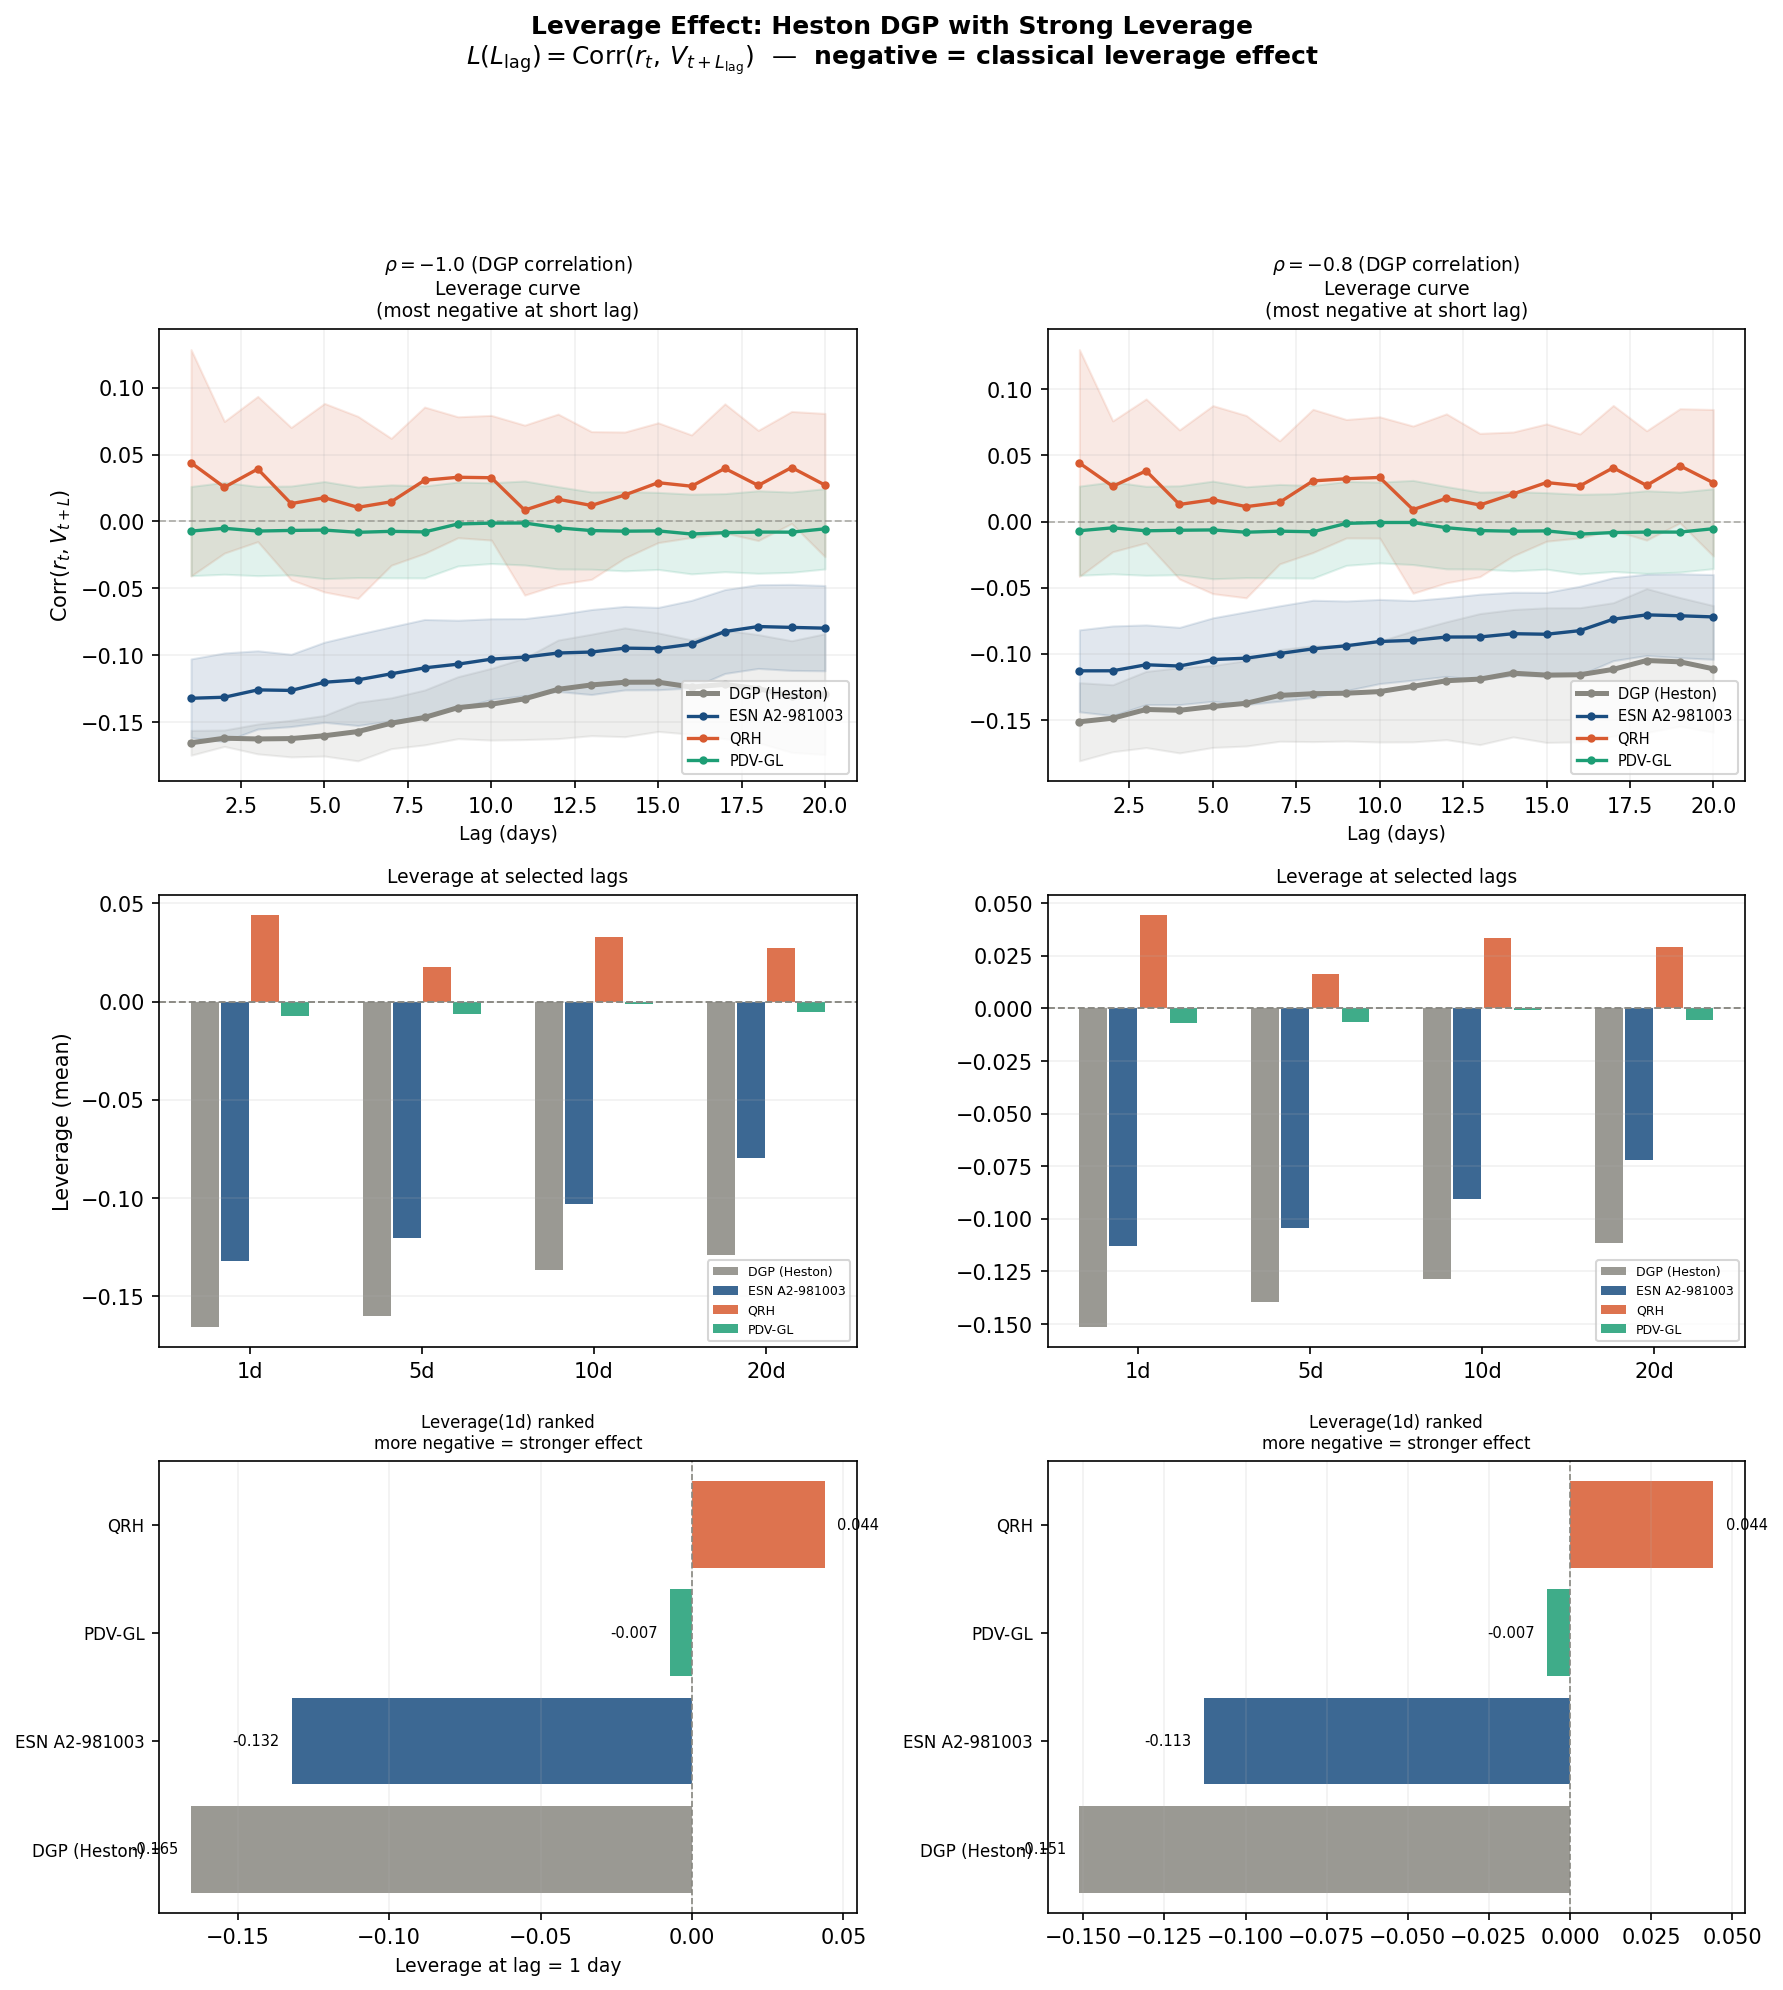
\includegraphics[width=0.85\textwidth]{heston_leverage_extreme_L1.png}
\caption{Leverage effect, one column per $\rho$ (left: perfect leverage $\rho=-1.00$; right: strong leverage $\rho=-0.80$): curve vs.\ lag (top), selected-lag bars (middle), and ranked 1-day comparison (bottom), for the DGP and all three calibrated models.}
\label{fig:L1}
\end{figure}

\begin{figure}[h]
\centering
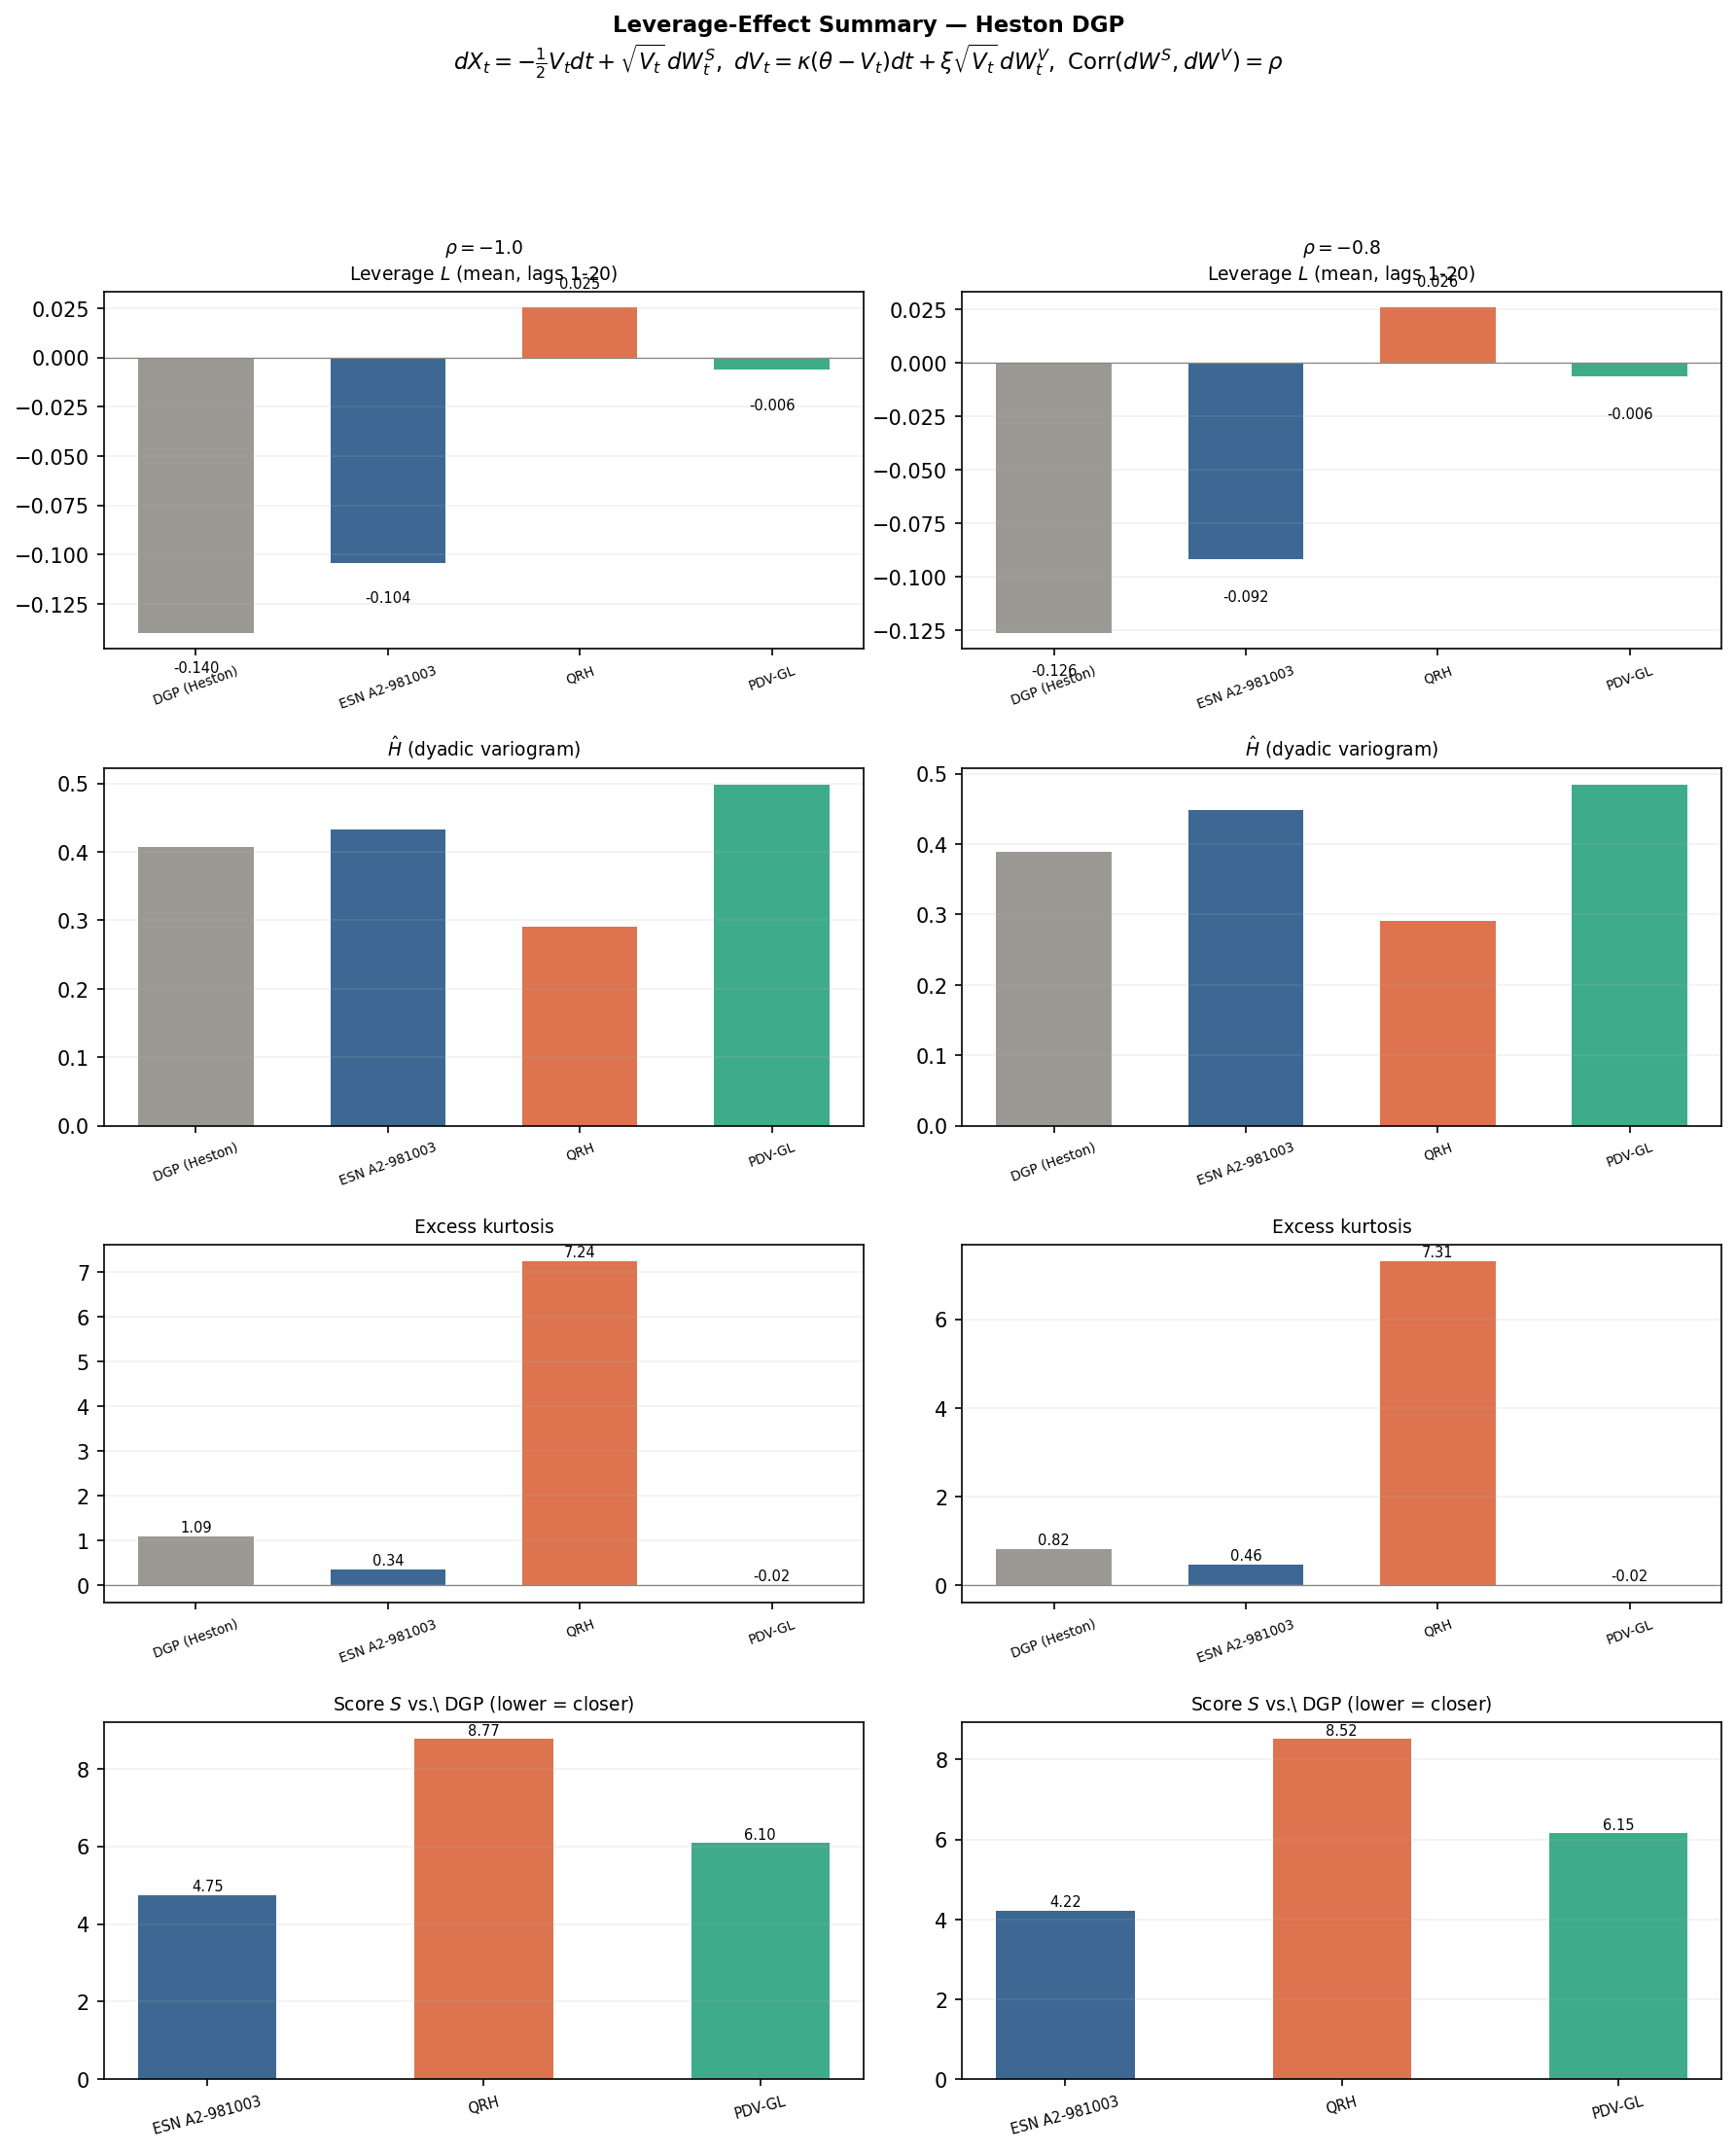
\includegraphics[width=0.85\textwidth]{heston_leverage_extreme_L2.png}
\caption{Summary at both $\rho$ values tested (columns: perfect leverage $\rho=-1.00$, strong leverage $\rho=-0.80$): leverage $L$ (top), $\hat H$ via dyadic variogram (second), excess kurtosis (third), and score $S$ vs.\ DGP (bottom).}
\label{fig:L2}
\end{figure}

\begin{figure}[h]
\centering
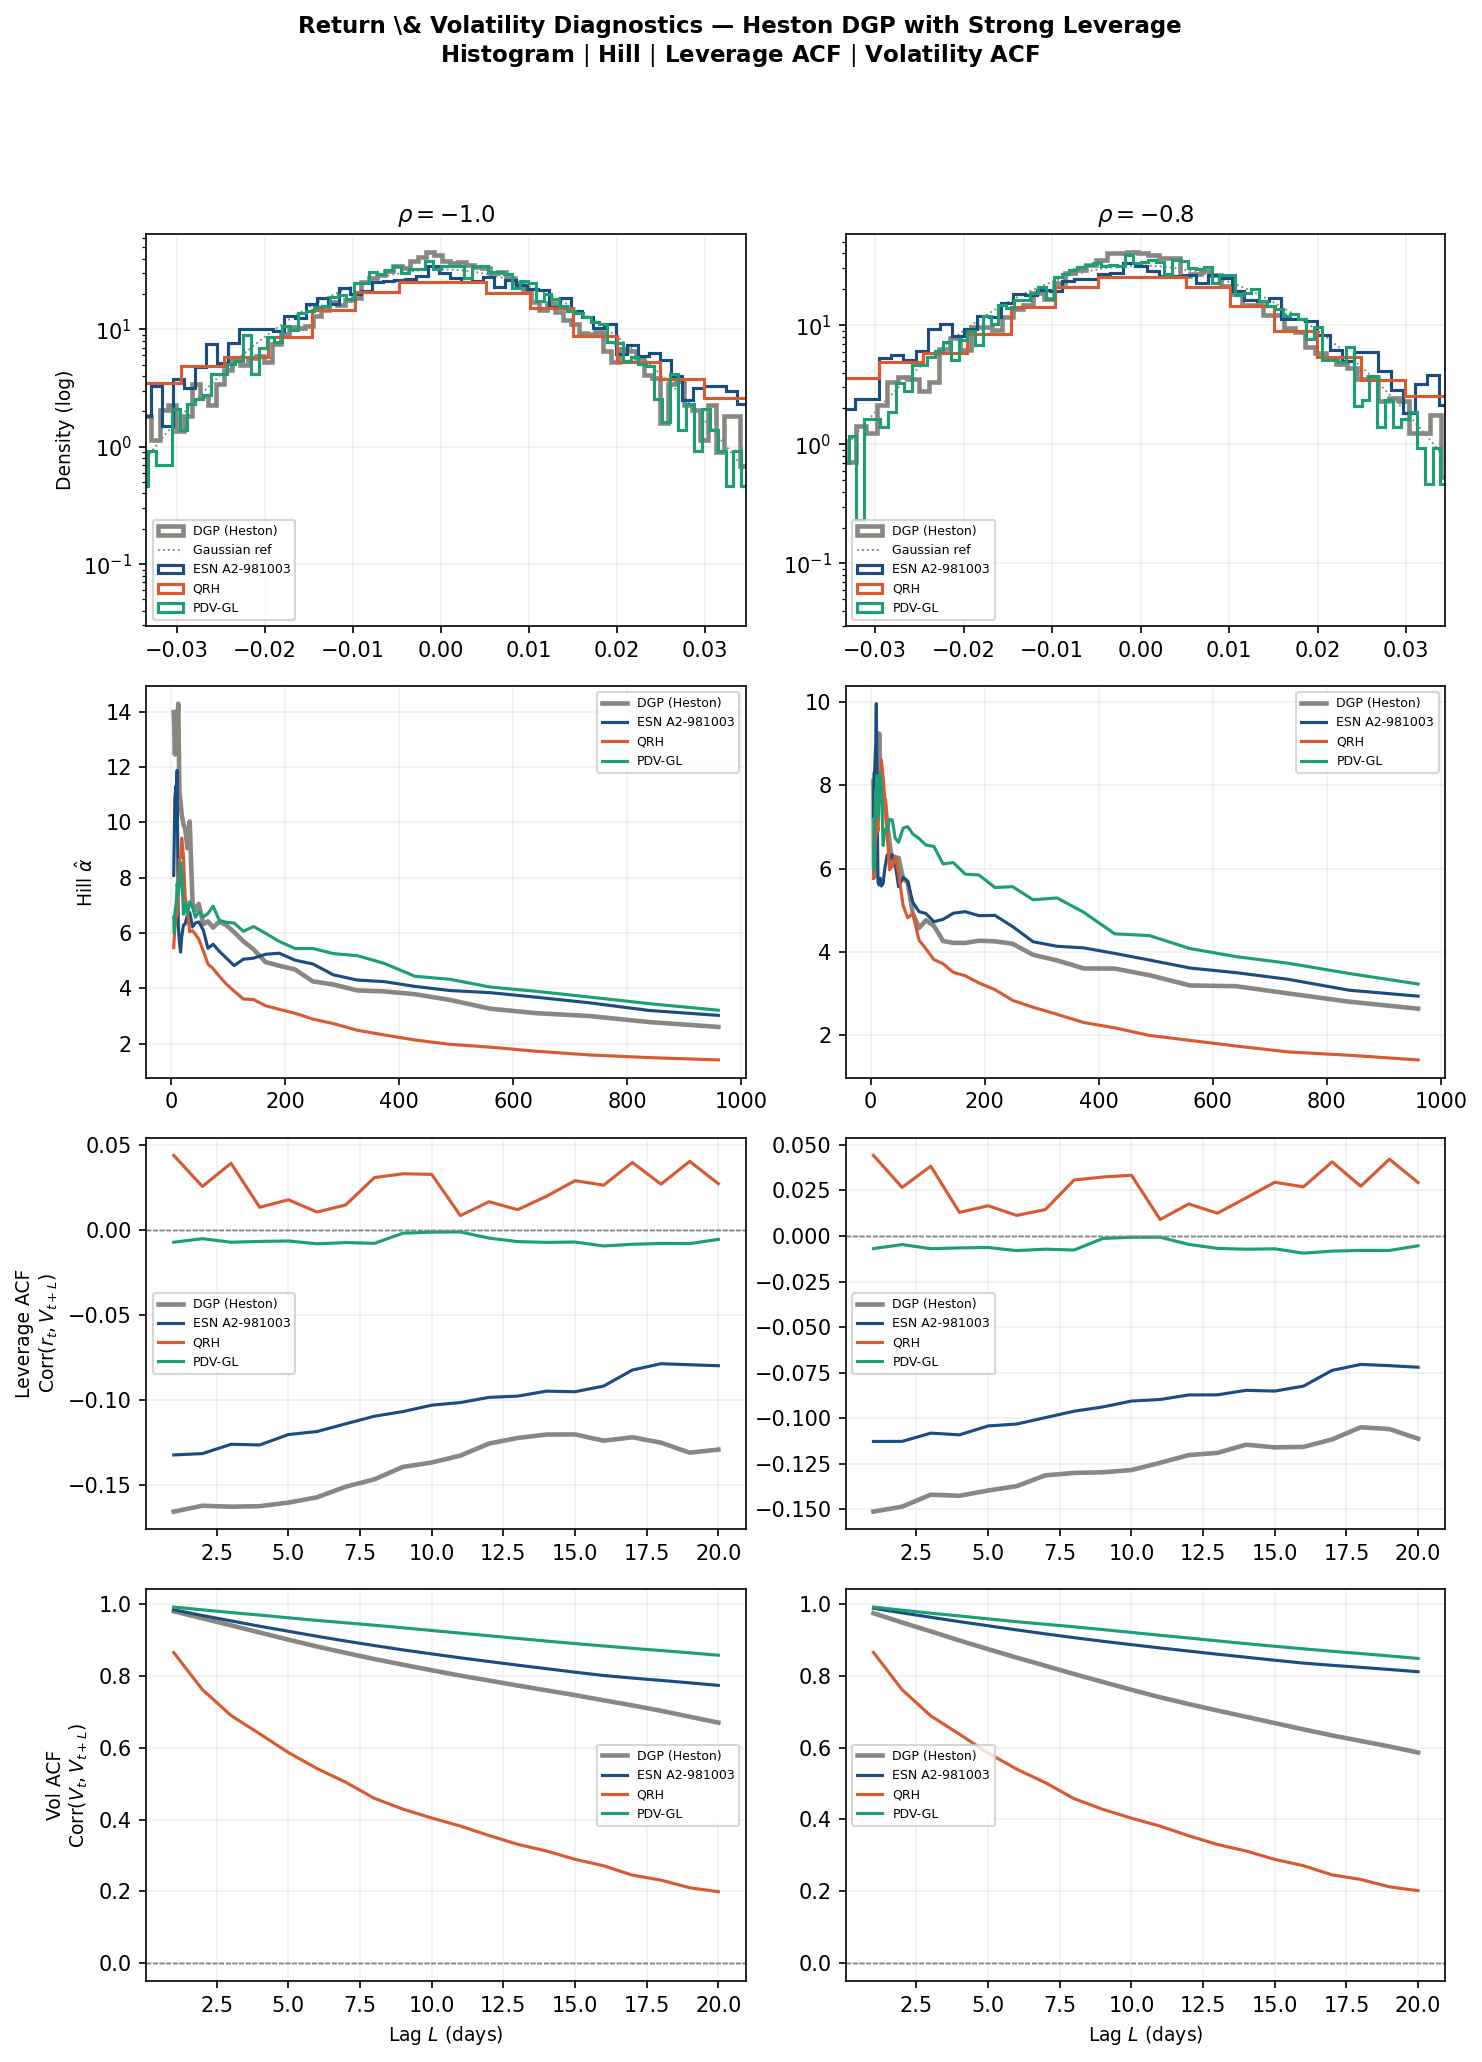
\includegraphics[width=0.95\textwidth]{heston_leverage_extreme_L3.png}
\caption{Return and volatility diagnostics, one column per $\rho$ (left: perfect leverage $\rho=-1.00$; right: strong leverage $\rho=-0.80$): log-density histogram vs.\ Gaussian reference (row 0); Hill estimator $\hat\alpha$ (row 1); leverage ACF $\mathrm{Corr}(r_t,V_{t+L})$ (row 2); volatility ACF $\mathrm{Corr}(V_t,V_{t+L})$ (row 3).}
\label{fig:L3}
\end{figure}

\section{Monte Carlo Setup}
\label{sec:mc}

\begin{center}\renewcommand{\arraystretch}{1.4}
\begin{tabular}{ll}\toprule Parameter & Value \\\midrule
DGP paths $n_{\rm dgp}$ & 30 \\
Calibration paths $n_{\rm cal}$ & 5 \\
Calibration trading days & 600 \\
Final paths $n_{\rm sim}$ & 30 \\
Final trading days & 2500 \\
Burn-in & 500 \\
$\Delta t$ (Heston, years) & $1/252$ \\
$\rho$ grid (DGP correlation) & $\{-1.00,\ -0.80\}$ \\
$\kappa,\theta,\xi$ (DGP, annualised) & $3.0,\ 0.04,\ 0.35$ \\
Feller condition $2\kappa\theta\geq\xi^2$ & $0.24\geq0.1225$ (satisfied) \\
Monte Carlo seed offset (this run) & $0$ (baseline seed) \\
\bottomrule\end{tabular}\end{center}

\begin{thebibliography}{9}
\bibitem{heston1993} S.L.\ Heston.
\textit{A closed-form solution for options with stochastic volatility}.
Rev.\ Fin.\ Studies 6(2), 1993.
\bibitem{bourgey2026} F.\ Bourgey, J.\ Gatheral.
\textit{Quadratic Rough Heston}. SSRN:5239929, 2026.
\bibitem{guyon2023} J.\ Guyon, J.\ Lekeufack.
\textit{Volatility is (mostly) path-dependent}. QF 23(9), 2023.
\end{thebibliography}
\end{document}
